\documentclass[tikz,border=8pt]{standalone}
\usepackage[T1]{fontenc}
\usepackage{helvet}
\renewcommand{\familydefault}{\sfdefault}
\usetikzlibrary{arrows.meta,positioning,fit,backgrounds,shapes.misc,calc}

\definecolor{cSrc}{HTML}{E8EEF7}
\definecolor{cEmb}{HTML}{DCEBDD}
\definecolor{cLlm}{HTML}{F6E7D0}
\definecolor{cHum}{HTML}{F3D9DC}
\definecolor{cArc}{HTML}{E6E0F0}
\definecolor{cOut}{HTML}{DDF0F0}
\definecolor{ink}{HTML}{22303C}

\tikzset{
  box/.style={draw=ink, rounded corners=3pt, line width=0.7pt, align=center,
              minimum width=3.3cm, minimum height=1.3cm, inner sep=5pt,
              font=\small, text=ink},
  src/.style={box, fill=cSrc},
  emb/.style={box, fill=cEmb},
  llm/.style={box, fill=cLlm},
  hum/.style={box, fill=cHum},
  arc/.style={box, fill=cArc},
  outp/.style={box, fill=cOut},
  flow/.style={-{Stealth[length=2.6mm]}, line width=0.9pt, color=ink},
  aux/.style={-{Stealth[length=2.2mm]}, line width=0.7pt, color=ink!70, dashed},
  lab/.style={font=\scriptsize\itshape, text=ink!80, align=center, inner sep=2pt},
  stage/.style={font=\scriptsize\bfseries, text=ink!60, inner sep=0pt},
}

\begin{document}
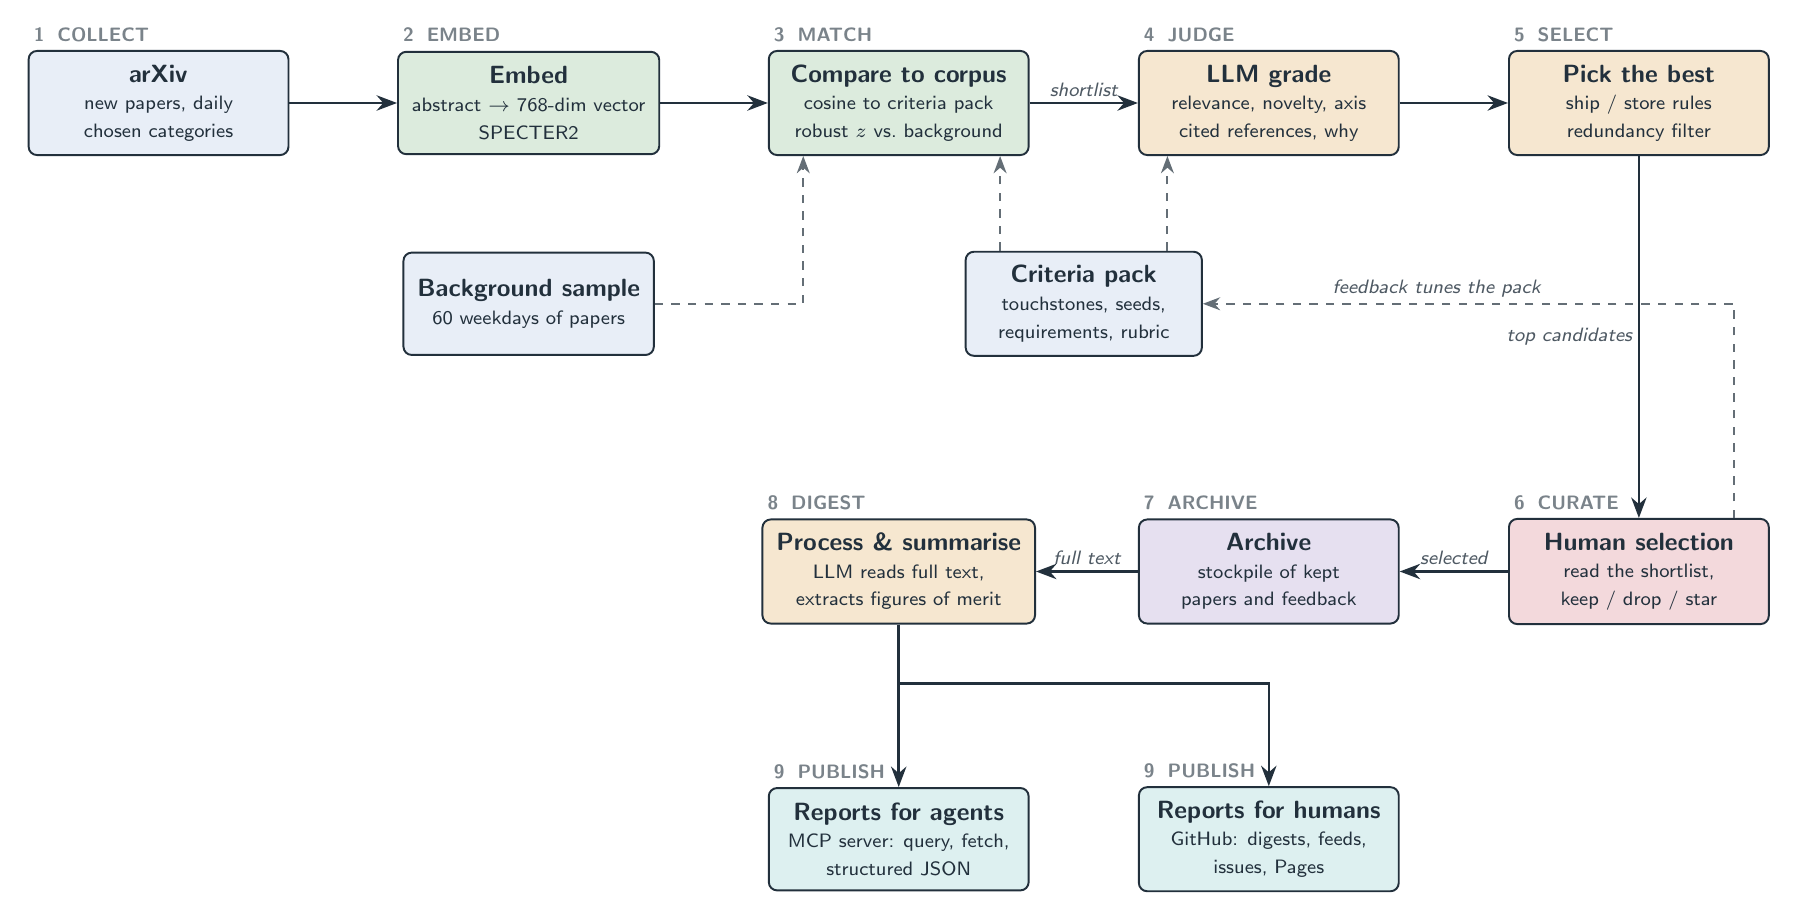
\begin{tikzpicture}
% grid: columns 4.7 cm apart, rows 3.4 cm apart
\def\cw{4.7}
\def\rh{3.4}

% ---- row 1: collect -> select --------------------------------------------
\node[src]  (arxiv)   at (0*\cw,0) {\textbf{arXiv}\\[-1pt]\scriptsize new papers, daily\\[-1pt]\scriptsize chosen categories};
\node[emb]  (embed)   at (1*\cw,0) {\textbf{Embed}\\[-1pt]\scriptsize abstract $\to$ 768-dim vector\\[-1pt]\scriptsize SPECTER2};
\node[emb]  (compare) at (2*\cw,0) {\textbf{Compare to corpus}\\[-1pt]\scriptsize cosine to criteria pack\\[-1pt]\scriptsize robust $z$ vs.\ background};
\node[llm]  (grade)   at (3*\cw,0) {\textbf{LLM grade}\\[-1pt]\scriptsize relevance, novelty, axis\\[-1pt]\scriptsize cited references, why};
\node[llm]  (pick)    at (4*\cw,0) {\textbf{Pick the best}\\[-1pt]\scriptsize ship / store rules\\[-1pt]\scriptsize redundancy filter};

% ---- middle band: reference material -------------------------------------
\node[src, minimum width=3.0cm] (bg)     at (1*\cw,-0.75*\rh) {\textbf{Background sample}\\[-1pt]\scriptsize 60 weekdays of papers};
\node[src, minimum width=3.0cm] (corpus) at (2.5*\cw,-0.75*\rh) {\textbf{Criteria pack}\\[-1pt]\scriptsize touchstones, seeds,\\[-1pt]\scriptsize requirements, rubric};

% ---- row 2: curate -> digest ---------------------------------------------
\node[hum]  (human)   at (4*\cw,-1.75*\rh) {\textbf{Human selection}\\[-1pt]\scriptsize read the shortlist,\\[-1pt]\scriptsize keep / drop / star};
\node[arc]  (archive) at (3*\cw,-1.75*\rh) {\textbf{Archive}\\[-1pt]\scriptsize stockpile of kept\\[-1pt]\scriptsize papers and feedback};
\node[llm]  (summ)    at (2*\cw,-1.75*\rh) {\textbf{Process \& summarise}\\[-1pt]\scriptsize LLM reads full text,\\[-1pt]\scriptsize extracts figures of merit};

% ---- row 3: outputs --------------------------------------------------------
\node[outp] (agents)  at (2*\cw,-2.75*\rh) {\textbf{Reports for agents}\\[-1pt]\scriptsize MCP server: query, fetch,\\[-1pt]\scriptsize structured JSON};
\node[outp] (humans)  at (3*\cw,-2.75*\rh) {\textbf{Reports for humans}\\[-1pt]\scriptsize GitHub: digests, feeds,\\[-1pt]\scriptsize issues, Pages};

% ---- main flow -------------------------------------------------------------
\draw[flow] (arxiv) -- (embed);
\draw[flow] (embed) -- (compare);
\draw[flow] (compare) -- node[lab, above] {shortlist} (grade);
\draw[flow] (grade) -- (pick);
\draw[flow] (pick) -- node[lab, left] {top candidates} (human);
\draw[flow] (human) -- node[lab, above] {selected} (archive);
\draw[flow] (archive) -- node[lab, above] {full text} (summ);
\draw[flow] (summ) -- (agents);
\draw[flow] (summ.south) -- ++(0,-0.75) -| (humans.north);

% ---- reference inputs (dashed) ---------------------------------------------
\draw[aux] (bg.east) -| ([xshift=0.45cm]compare.south west);
\draw[aux] ([xshift=0.45cm]corpus.north west) -- ([xshift=0.45cm]corpus.north west |- compare.south);
\draw[aux] ([xshift=-0.45cm]corpus.north east) -- ([xshift=-0.45cm]corpus.north east |- grade.south);
% feedback loop: human choices retune the pack
\draw[aux] ([xshift=-0.45cm]human.north east) |- node[lab, above, pos=0.78] {feedback tunes the pack} (corpus.east);

% ---- stage captions ----------------------------------------------------------
\foreach \n/\t in {arxiv/{1\; COLLECT}, embed/{2\; EMBED}, compare/{3\; MATCH},
                   grade/{4\; JUDGE}, pick/{5\; SELECT}, human/{6\; CURATE},
                   archive/{7\; ARCHIVE}, summ/{8\; DIGEST}}
  \node[stage, anchor=south west] at ([xshift=2pt,yshift=3pt]\n.north west) {\t};
\node[stage, anchor=south west] at ([xshift=2pt,yshift=3pt]agents.north west) {9\; PUBLISH};
\node[stage, anchor=south west] at ([xshift=2pt,yshift=3pt]humans.north west) {9\; PUBLISH};

\end{tikzpicture}
\end{document}
